\documentclass[12pt,letterpaper]{article}

% --- Paquetes Básicos ---
\usepackage[utf8]{inputenc}
\usepackage[spanish,es-tabla]{babel}
\usepackage{geometry}
\geometry{top=2.5cm, bottom=2.5cm, left=3cm, right=3cm}
\usepackage{graphicx}
\usepackage{booktabs}
\usepackage{amsmath}
\usepackage{amsfonts}
\usepackage{float}
\usepackage{caption}
\usepackage{subcaption}
\usepackage{fancyhdr}
\usepackage{hyperref}
\usepackage{listings}
\usepackage{xcolor}
\usepackage{longtable}
\usepackage{enumitem}
\usepackage{textcomp}
% \usepackage[backend=bibtex]{biblatex} % No usado - sin bibliografia externa

% --- Configuración de Hipervínculos ---
\hypersetup{
    colorlinks=true,
    linkcolor=blue,
    filecolor=magenta,
    urlcolor=cyan,
    pdftitle={SmartHome IoT — Informe Unidad 2},
    pdfpagemode=FullScreen,
}

% --- Configuración de listings (Código Fuente) ---
\definecolor{codegreen}{rgb}{0,0.6,0}
\definecolor{codegray}{rgb}{0.5,0.5,0.5}
\definecolor{codepurple}{rgb}{0.58,0,0.82}
\definecolor{backcolour}{rgb}{0.95,0.95,0.92}

\lstdefinestyle{mystyle}{
    backgroundcolor=\color{backcolour},
    commentstyle=\color{codegreen},
    keywordstyle=\color{blue},
    numberstyle=\tiny\color{codegray},
    stringstyle=\color{codepurple},
    basicstyle=\ttfamily\footnotesize,
    breakatwhitespace=false,
    breaklines=true,
    captionpos=b,
    keepspaces=true,
    numbers=left,
    numbersep=5pt,
    showspaces=false,
    showstringspaces=false,
    showtabs=false,
    tabsize=2
}
\lstset{style=mystyle}
\lstset{
    inputencoding=utf8,
    extendedchars=true,
    literate={á}{{\'a}}1 {é}{{\'e}}1 {í}{{\'i}}1 {ó}{{\'o}}1 {ú}{{\'u}}1
             {ñ}{{\~n}}1 {ü}{{\"u}}1
             {Á}{{\'A}}1 {É}{{\'E}}1 {Í}{{\'I}}1 {Ó}{{\'O}}1 {Ú}{{\'U}}1
             {Ñ}{{\~N}}1
             {°}{{\textdegree}}1
             {€}{{\texteuro}}1
             {—}{---}1 {–}{--}1
             {“}{``}1 {”}{''}1
}

% --- Encabezado y Pie de Página ---
\pagestyle{fancy}
\fancyhf{}
\lhead{SmartHome IoT - Informe Técnico Unidad 2}
\rhead{Equipo 69}
\lfoot{Universidad de Talca}
\rfoot{\thepage}
\renewcommand{\headrulewidth}{0.4pt}
\renewcommand{\footrulewidth}{0.4pt}

% --- Inicio del Documento ---
\begin{document}

% ==========================================
% PORTADA
% ==========================================
\begin{titlepage}
    \centering
    \vspace*{1cm}
    {\scshape\LARGE Universidad de Talca \par}
    {\scshape\Large Facultad de Ingeniería \par}
    {\scshape\large Escuela de Ingeniería Civil en Computación \par}
    \vspace{1.5cm}
    {\huge\bfseries SmartHome IoT: Seguridad, LLM Local y Agente Autónomo\par}
    \vspace{0.5cm}
    {\Large\itshape Informe Técnico — Unidad 2 (Equipo 69)\par}
    \vspace{2cm}

    \begin{tabular}{rl}
        \textbf{Asignatura:} & Internet de las Cosas \\
        \textbf{Profesor:} & Ricardo Pérez \\
        \textbf{Fecha:} & Junio 2026 \\
    \end{tabular}

    \vspace{1.5cm}
    {\large\textbf{Integrantes:}\par}
    \begin{tabular}{rl}
        Mariano Muñoz R. & \mbox{\texttt{mariano.munoz@alumnos.utalca.cl}} \\
        Cristian Ruiz I. & \mbox{\texttt{cristian.ruiz@alumnos.utalca.cl}} \\
        Camilo Fuentes G. & \mbox{\texttt{camilo.fuentes@alumnos.utalca.cl}} \\
    \end{tabular}

    \vfill
    {\large \today \par}
\end{titlepage}

\newpage

% ==========================================
% ÍNDICE
% ==========================================
\tableofcontents
\newpage

% ==========================================
% LISTA DE FIGURAS Y TABLAS
% ==========================================
\listoffigures
\listoftables
\newpage

% ==========================================
% 1. INTRODUCCIÓN
% ==========================================
\section{Introducción}

En la Unidad 1 del proyecto se estableció la infraestructura base de comunicación MQTT con un broker Mosquitto en texto plano, la integración de sensores/actuadores con Arduino MKR1000 y ESP32-CAM, y un sistema de reconocimiento facial para control de acceso. Sobre esa base, la Unidad 2 añade tres pilares fundamentales:

\begin{enumerate}
    \item \textbf{Seguridad en las comunicaciones:} Migración de MQTT texto plano a TLS con autenticación por usuario/contraseña y políticas de control de acceso (ACL) granulares para cada dispositivo.
    \item \textbf{LLM Local:} Integración de un modelo de lenguaje pequeño (phi3:mini vía Ollama) como cerebro del hogar, capaz de analizar contexto sensorial y decidir acciones.
    \item \textbf{Agente Autónomo:} Implementación de un agente LangGraph con 15 nodos que monitoriza el hogar, evalúa umbrales, consulta el LLM cuando es necesario y ejecuta acciones de forma segura a través de un servidor MCP.
\end{enumerate}

Este informe detalla la arquitectura, implementación y resultados de cada uno de estos componentes, incluyendo un análisis de vulnerabilidades y una reflexión crítica sobre el uso de LLMs en entornos de producción IoT.

\newpage

% ==========================================
% 2. INFRAESTRUCTURA Y SEGURIDAD MQTT
% ==========================================
\section{Infraestructura y Seguridad MQTT}

\subsection{Arquitectura General}

La Figura \ref{fig:arqui_u2} muestra la arquitectura completa de la Unidad 2. El broker Mosquitto actúa como bus central de comunicación, con dos listeners diferenciados:

\begin{itemize}
    \item \textbf{Puerto 8883 (TLS):} Para servicios internos Docker (Node-RED, Backend, LLM Gateway, Digital Twin, MCP Server).
    \item \textbf{Puerto 1884 (plain + auth):} Para placas embebidas (MKR1000, ESP32-CAM) cuyo hardware no soporta TLS moderno.
\end{itemize}

\begin{figure}[H]
    \centering
    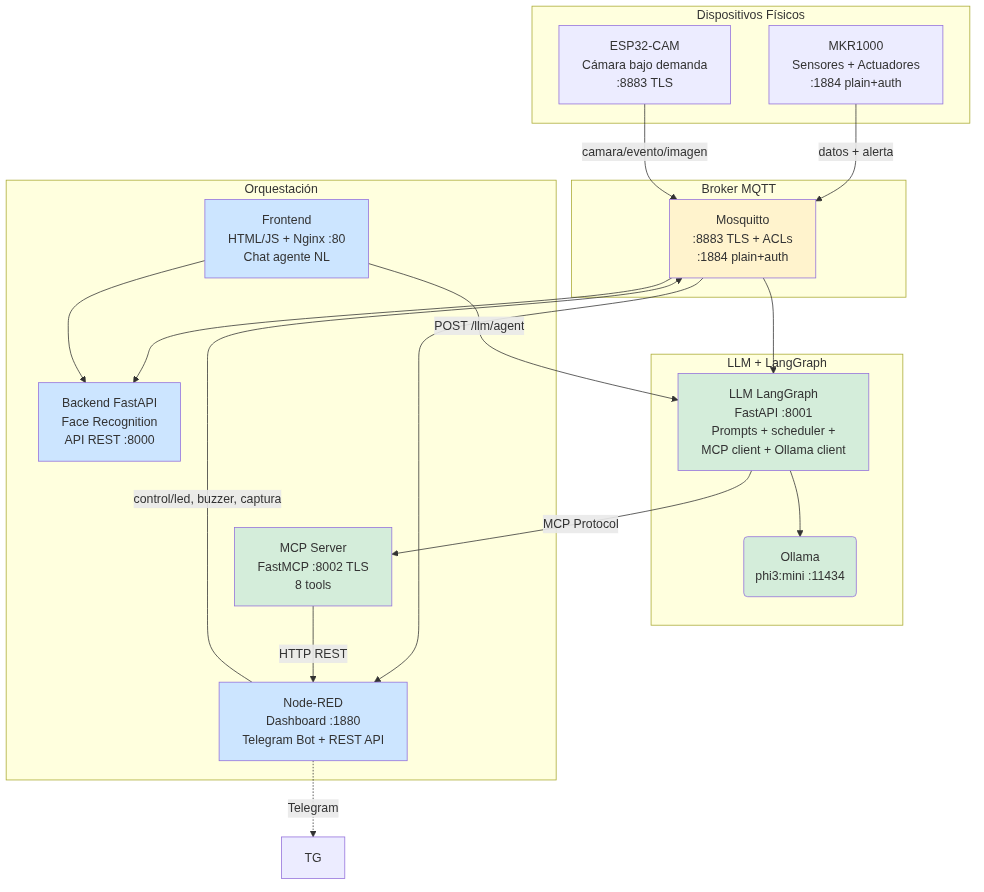
\includegraphics[width=\textwidth]{img/arqui_u2.png}
    \caption{Arquitectura del sistema en Unidad 2, mostrando los componentes de seguridad, LLM y agente autónomo.}
    \label{fig:arqui_u2}
\end{figure}

\bigskip
\subsection{Configuración TLS}

El archivo \mbox{\texttt{mosquitto.conf}} define tres listeners con diferentes niveles de seguridad. El Listado \ref{lst:mosquitto_conf} muestra la configuración completa.

\begin{lstlisting}[language={}, label=lst:mosquitto_conf, caption={Configuración de Mosquitto con TLS y ACLs por listener.}]
# TLS listener — servicios internos
listener 8883 0.0.0.0
cafile /mosquitto/certs/ca.crt
certfile /mosquitto/certs/server.crt
keyfile /mosquitto/certs/server.key
require_certificate false
password_file /mosquitto/config/passwd
acl_file /mosquitto/config/acl.conf
allow_anonymous false

# Non-TLS listener — placas embebidas
listener 1884 0.0.0.0
password_file /mosquitto/config/passwd
acl_file /mosquitto/config/acl.conf
allow_anonymous false

# Healthcheck listener — localhost only
listener 1883 127.0.0.1
allow_anonymous true
\end{lstlisting}

\subsection{Generación de Certificados}

Los certificados TLS se generan mediante el script \mbox{\texttt{generate-certs.sh}}, que crea una Autoridad Certificadora (CA) autofirmada con validez de 365 días y firma los certificados del servidor y del MCP Server. El script \mbox{\texttt{sync-ca-to-firmware.sh}} sincroniza el CA cert con el firmware de la ESP32-CAM para que pueda validar la conexión TLS.

Un aspecto crítico del diseño es que la ESP32-CAM requiere sincronización NTP para validar la fecha del certificado, ya que el chip ESP32 no tiene RTC con batería de respaldo.

\begin{table}[H]
    \centering
    \caption{Archivos de certificados TLS generados.}
    \label{tab:certificados}
    \begin{tabular}{lll}
        \toprule
        \textbf{Archivo} & \textbf{Rol} & \textbf{Ubicación} \\
        \midrule
        \mbox{\texttt{ca.crt}} / \mbox{\texttt{ca.key}} & Autoridad Certificadora & \mbox{\texttt{deploy/mosquitto/certs/}} \\
        \mbox{\texttt{server.crt}} / \mbox{\texttt{server.key}} & Certificado del broker & \mbox{\texttt{deploy/mosquitto/certs/}} \\
        \mbox{\texttt{mcp-server.crt}} / \mbox{\texttt{mcp-server.key}} & Certificado MCP Server & \mbox{\texttt{deploy/mosquitto/certs/}} \\
        \bottomrule
    \end{tabular}
\end{table}

\bigskip
\subsection{Autenticación y Control de Acceso (ACL)}

Se implementaron seis usuarios MQTT, cada uno con permisos estrictamente limitados a los tópicos necesarios para su función. El Cuadro \ref{tab:usuarios_mqtt} resume los perfiles y sus permisos.

\begin{table}[H]
    \centering
    \caption{Usuarios MQTT y sus permisos ACL.}
    \label{tab:usuarios_mqtt}
    \small
    \begin{tabular}{p{4cm}p{6cm}l}
        \toprule
        \textbf{Usuario} & \textbf{Permisos} & \textbf{Rol} \\
        \midrule
        \mbox{\texttt{mkr1000-equipo69}} & Write: \mbox{\texttt{datos}}, \mbox{\texttt{alerta}} & Publicar sensores \\
        & Read: \mbox{\texttt{control/led}}, \mbox{\texttt{control/led-puerta}} & Recibir comandos \\
        \midrule
        \mbox{\texttt{esp32cam-equipo69}} & Write: \mbox{\texttt{camara/evento}}, \mbox{\texttt{camara/imagen}} & Publicar imágenes \\
        & Read: \mbox{\texttt{camara/captura}} & Recibir órdenes \\
        \midrule
        \mbox{\texttt{backend-equipo69}} & Write: \mbox{\texttt{acceso/*}}, \mbox{\texttt{control/led-puerta}} & Control acceso \\
        & Read: \mbox{\texttt{camara/imagen}}, \mbox{\texttt{camara/url}} & Procesar imágenes \\
        \midrule
        \mbox{\texttt{nodered-smarthome}} & Write: \mbox{\texttt{control/*}}, \mbox{\texttt{camara/captura}} & Orquestador \\
        & Read: \mbox{\texttt{smarthome/+/datos}}, \mbox{\texttt{llm/decision}} & Monitoreo \\
        \midrule
        \mbox{\texttt{llm-gateway-equipo69}} & Write: \mbox{\texttt{llm/decision}} & Solo publicar decisiones \\
        & (sin read) & \\
        \midrule
        \mbox{\texttt{digital-twin-equipo69}} & Read: \mbox{\texttt{smarthome/equipo69/\#}} & Estado completo \\
        & Write: \mbox{\texttt{prediccion/*}} & Publicar predicciones \\
        \bottomrule
    \end{tabular}
\end{table}

Nótese que el usuario \mbox{\texttt{llm-gateway-equipo69}} NO tiene permisos de escritura en ningún tópico de control (\mbox{\texttt{control/led}}, \mbox{\texttt{control/led-puerta}}, etc.). Esto es intencional: el LLM nunca publica directamente comandos a los actuadores. Node-RED actúa como gatekeeper, recibiendo las decisiones del LLM y decidiendo si ejecutarlas o no.

\begin{lstlisting}[language={}, label=lst:acl_llm, caption={Extracto de \mbox{\texttt{acl.conf}} mostrando las restricciones del LLM Gateway.}]
# LLM Gateway — reasoning decisions only (publish-only, no subscribe)
user llm-gateway-equipo69
topic write smarthome/equipo69/llm/decision
\end{lstlisting}

\subsection{Consideración de Seguridad: Puerto 1883}

Si bien la especificación solicita deshabilitar completamente el puerto 1883 en texto plano, en nuestra implementación este puerto permanece activo pero restringido exclusivamente a \mbox{\texttt{127.0.0.1}} (localhost) para permitir el healthcheck de Docker sobre Mosquitto. Dado que no es accesible desde la red externa y no requiere autenticación, representa un riesgo mínimo controlado. Esta decisión de diseño se tomó para mantener la capacidad de orquestación sin comprometer la seguridad perimetral.

\newpage

% ==========================================
% 3. FIRMWARE IoT CON TLS
% ==========================================
\section{Actualización de Firmware con Soporte TLS}

\subsection{ESP32-CAM: Conexión Segura}

El firmware de la ESP32-CAM se actualizó para usar \mbox{\texttt{WiFiClientSecure}} con certificado CA embebido. El flujo de conexión es:

\begin{enumerate}
    \item Conectar a WiFi.
    \item Sincronizar hora vía NTP (necesario para validar la fecha del certificado TLS).
    \item Configurar \mbox{\texttt{WiFiClientSecure.setCACert()}} con el CA cert del proyecto.
    \item Conectar al broker Mosquitto en puerto 8883.
    \item Publicar evento \mbox{\texttt{camara/evento}} con \texttt{\{"status":"camara\_lista"\}}.
\end{enumerate}

El CA cert se inyecta automáticamente en el firmware mediante el script \mbox{\texttt{sync-ca-to-firmware.sh}}, que extrae el certificado del contenedor Docker de Mosquitto y lo inserta en el archivo \mbox{\texttt{secrets.h}} de la ESP32-CAM.

\subsection{Externalización de Credenciales}

Ambos firmwares utilizan el patrón \mbox{\texttt{secrets.h.example}} + \mbox{\texttt{secrets.h}} (en \mbox{\texttt{.gitignore}}) para mantener las credenciales fuera del repositorio. Los templates contienen valores placeholder que el desarrollador debe reemplazar antes de flashear.

\subsection{Lógica de Reconexión}

Ambos firmwares implementan reconexión automática con backoff exponencial:

\begin{itemize}
    \item \textbf{MKR1000} (\mbox{\texttt{mqtt\_manager.cpp}}): Reintenta conexión MQTT cada 5 segundos si se pierde la conexión. Reintenta WiFi cada 10 segundos si se cae la red.
    \item \textbf{ESP32-CAM} (\mbox{\texttt{mqtt\_bridge.cpp}}): Similar, con reintentos cada 5 segundos para MQTT y 10 segundos para WiFi.
\end{itemize}

\newpage

% ==========================================
% 4. LLM LOCAL Y GATEWAY
% ==========================================
\section{LLM Local e Integración}

\subsection{Ollama + phi3:mini}

Ollama se ejecuta en un contenedor Docker con el modelo \mbox{\texttt{phi3:mini}} (3.8B parámetros). Se configuró con:

\begin{itemize}
    \item \mbox{\texttt{OLLAMA\_KEEP\_ALIVE=-1}}: Mantiene el modelo cargado en memoria para evitar tiempos de carga fría.
    \item \mbox{\texttt{OLLAMA\_NUM\_THREADS=6}}: Paralelismo para CPU (sin GPU).
    \item Límite de memoria: 4 GB.
\end{itemize}

\subsection{LLM Gateway (FastAPI)}

El LLM Gateway es un microservicio FastAPI en el puerto \mbox{\texttt{:8001}} que centraliza todas las interacciones con Ollama. Sus responsabilidades incluyen:

\begin{itemize}
    \item \textbf{Decisión de seguridad:} Toma el contexto actual de sensores (temperatura, humedad, gas, ruido), construye un prompt dinámico y consulta a Ollama para determinar el nivel de alerta.
    \item \textbf{Forzado de formato JSON:} La petición HTTP a Ollama incluye \mbox{\texttt{"format": "json"}} para obligar al modelo a devolver una estructura parseable. El Listado \ref{lst:ollama_format} muestra la configuración en \mbox{\texttt{ollama\_client.py}}.
    \item \textbf{Gestión de errores:} Timeout estricto de 3 segundos para decisiones, con retry exponencial y fallback determinístico si el LLM no responde.
    \item \textbf{Scheduler del agente:} Ejecuta el ciclo autónomo del LangGraph Agent cada 30 segundos.
    \item \textbf{Endpoint REST:} Expone \mbox{\texttt{POST /llm/agent}} para consultas del usuario desde el frontend.
\end{itemize}

\begin{lstlisting}[language=Python, label=lst:ollama_format, caption={Forzado de formato JSON en las peticiones a Ollama.}]
payload = {
    "model": self.model,
    "prompt": prompt,
    "stream": False,
}
if format_json:
    payload["format"] = "json"  # Obliga a Ollama a devolver JSON
if system_prompt is not None:
    payload["system"] = system_prompt
\end{lstlisting}

\subsection{Prompts Dinámicos}

El prompt de decisión se construye en tiempo real inyectando los valores actuales de los sensores. El Listado \ref{lst:prompt_builder} muestra el sistema de prompts.

\begin{lstlisting}[language=Python, label=lst:prompt_builder, caption={Constructor de prompts dinámicos para decisión de seguridad.}]
system_prompt = (
    "Sos el agente de seguridad de una casa inteligente (SmartHome equipo69).\n"
    "Tu tarea es analizar los datos de sensores y determinar el nivel de alerta.\n\n"
    "Niveles de alerta:\n"
    "- critico: gas > 1020 ppm o temperatura > 30 °C (emergencia)\n"
    "- alto: gas > 800 ppm o temperatura > 28 °C (riesgo significativo)\n"
    "- medio: gas > 400 ppm o ruido > 85 dB (precaución)\n"
    "- bajo: valores levemente fuera de rango\n"
    "- info: todo normal\n\n"
    "Respondé SOLO con un JSON en este formato exacto:\n"
    '{"nivel": "critico|alto|medio|bajo|info", '
    '"razonamiento": "explicación en español", '
    '"acciones": [{"tool": "nombre", "args": {...}}], '
    '"confidence": 0.0-1.0}'
)
\end{lstlisting}

\subsection{Manejo de Errores y Fallback Determinístico}

El sistema implementa una estrategia de tolerancia a fallos en cascada para el LLM:

\begin{enumerate}
    \item \textbf{Timeout:} La llamada a Ollama tiene un timeout de 3 segundos envuelto en \mbox{\texttt{asyncio.wait\_for}}.
    \item \textbf{Retry exponencial:} \mbox{\texttt{httpx.AsyncClient}} con backoff $2^{attempt}$ segundos (1s, 2s, 4s, ...).
    \item \textbf{Fallback determinístico:} Si el LLM falla o devuelve JSON inválido, se llama a \mbox{\texttt{\_deterministic\_fallback()}} para aplicar reglas fijas (Cuadro \ref{tab:fallback}).
\end{enumerate}

\begin{table}[H]
    \centering
    \caption{Lógica del fallback determinístico cuando el LLM no está disponible.}
    \label{tab:fallback}
    \begin{tabular}{lc}
        \toprule
        \textbf{Condición} & \textbf{Acción} \\
        \midrule
        Gas $>$ 1020 ppm o Temp $>$ 30$^{\circ}$C & Nivel crítico: LED alerta + Telegram \\
        Gas $>$ 800 ppm o Temp $>$ 28$^{\circ}$C & Nivel alto: solo Telegram \\
        Gas $>$ 400 ppm & Nivel medio: solo Telegram \\
        Valores normales & Nivel normal: sin acciones \\
        \bottomrule
    \end{tabular}
\end{table}

\newpage

% ==========================================
% 5. MCP SERVER
% ==========================================
\section{Servidor MCP (Model Context Protocol)}

El MCP Server es un servicio Python independiente que implementa el protocolo MCP sobre Streamable HTTP con TLS en el puerto \mbox{\texttt{:8002}}. Expone 8 herramientas (tools) que encapsulan las operaciones del hogar inteligente.

\subsection{Tools Disponibles}

\small
\setlength{\LTleft}{0pt plus 1fill}
\setlength{\LTright}{0pt plus 1fill}
\begin{longtable}{p{3.5cm}p{2cm}p{7cm}}
    \caption{Tools MCP disponibles para el agente LangGraph.} \\
    \toprule
    \textbf{Tool} & \textbf{Tipo} & \textbf{Descripción} \\
    \midrule
    \endfirsthead
    \caption[]{Tools MCP (continuación)} \\
    \toprule
    \textbf{Tool} & \textbf{Tipo} & \textbf{Descripción} \\
    \midrule
    \endhead
    \bottomrule
    \endfoot
    \mbox{\texttt{get\_sensor\_state}} & Info & Temperatura, humedad, gas, sonido actuales \\
    \mbox{\texttt{get\_system\_status}} & Info & Estado lógico de LED y alertas \\
    \mbox{\texttt{query\_history}} & Info & Historial CSV con filtro temporal \\
    \mbox{\texttt{activate\_led\_alerta}} & Acción & Encender/apagar LED de alerta \\
    \mbox{\texttt{activate\_led\_puerta}} & Acción & Encender/apagar LED de puerta \\
    \mbox{\texttt{send\_notification}} & Acción & Enviar mensaje por Telegram \\
    \mbox{\texttt{silence\_alerts}} & Acción & Apagar todas las alertas \\
    \mbox{\texttt{trigger\_camera}} & Acción & Disparar captura de cámara \\
\end{longtable}
\setlength{\LTleft}{0pt}
\setlength{\LTright}{0pt}

\subsection{Flujo de Comunicación}

El MCP Server nunca se conecta directamente al broker MQTT. En su lugar, traduce llamadas MCP a peticiones HTTP REST hacia Node-RED, que es el único componente autorizado para publicar en tópicos de control MQTT:

{\footnotesize
\begin{verbatim}
LangGraph → MCP Sidecar (:8002, TLS)
  → HTTP → Node-RED REST (:1880)
  → MQTT → dispositivos
\end{verbatim}
}

Este diseño garantiza que el LLM (o cualquier cliente MCP) nunca tenga acceso directo a los actuadores físicos, cumpliendo con el principio de mínimo privilegio.

\newpage

% ==========================================
% 6. LANGGRAPH AGENT
% ==========================================
\section{Agente Autónomo LangGraph}

\subsection{Arquitectura del Grafo}

El agente se implementa como un StateGraph de LangGraph con 15 nodos interconectados mediante aristas condicionales. La Figura \ref{fig:langgraph_flow} muestra el diagrama de flujo completo.

\begin{figure}[H]
    \centering
    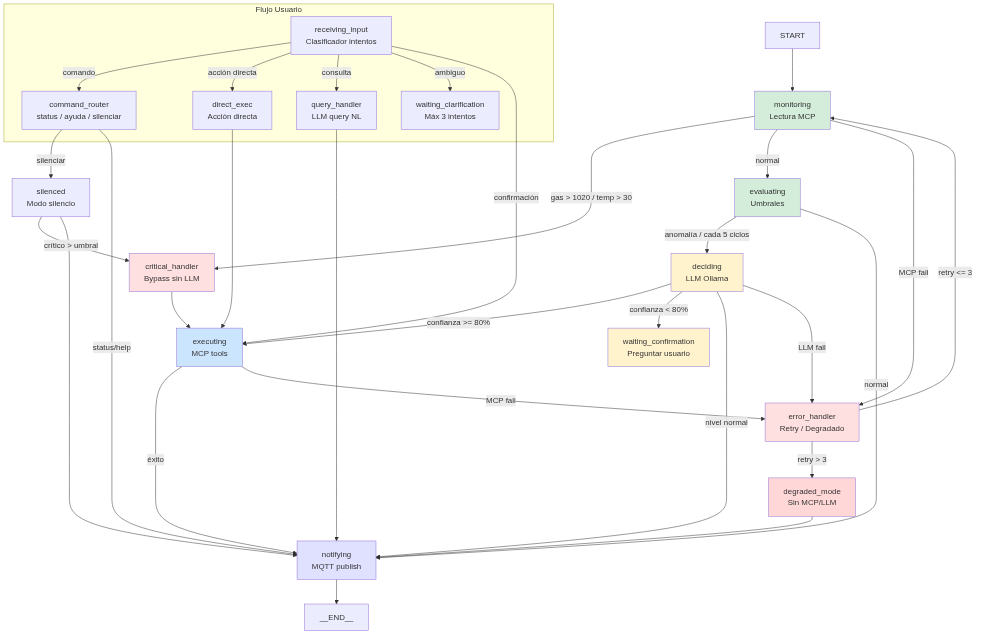
\includegraphics[width=\textwidth]{img/langgraph_flow.png}
    \caption{Diagrama de flujo del agente LangGraph con 15 nodos y rutas de decisión.}
    \label{fig:langgraph_flow}
\end{figure}

\subsection{Descripción de Nodos}

\small
\setlength{\LTleft}{0pt plus 1fill}
\setlength{\LTright}{0pt plus 1fill}
\begin{longtable}{p{3.5cm}p{2.5cm}p{6.5cm}}
    \caption{Nodos del StateGraph LangGraph.} \\
    \toprule
    \textbf{Nodo} & \textbf{Entrada} & \textbf{Función} \\
    \midrule
    \endfirsthead
    \caption[]{Nodos LangGraph (continuación)} \\
    \toprule
    \textbf{Nodo} & \textbf{Entrada} & \textbf{Función} \\
    \midrule
    \endhead
    \bottomrule
    \endfoot
    \mbox{\texttt{monitoring}} & MCP sensors & Lee datos de sensores vía MCP. Detecta staleness. \\
    \mbox{\texttt{evaluating}} & Sensor data & Evalúa umbrales: anomalía, tendencia ascendente. \\
    \mbox{\texttt{critical\_handler}} & Umbral crítico & Bypass crítico SIN LLM: plan fijo de acciones. \\
    \mbox{\texttt{deciding}} & Contexto sensors & Consulta a Ollama para decisión. Timeout 3s. \\
    \mbox{\texttt{executing}} & Acciones plan & Ejecuta secuencialmente vía MCP. \\
    \mbox{\texttt{notifying}} & Decisión & Prepara payload y publica a MQTT. \\
    \mbox{\texttt{error\_handler}} & Error & Retry (máx 3) o modo degradado. \\
    \mbox{\texttt{degraded\_mode}} & Error persistente & Desactiva MCP, notifica al usuario. \\
    \mbox{\texttt{receiving\_input}} & Usuario texto & Clasifica intent con reglas + LLM. \\
    \mbox{\texttt{command\_router}} & Intento & /status, /ayuda, silenciar. \\
    \mbox{\texttt{query\_handler}} & Consulta NL & Responde preguntas con LLM + datos MCP. \\
    \mbox{\texttt{direct\_exec}} & Acción directa & Keywords → herramienta MCP. \\
    \mbox{\texttt{waiting\_confirmation}} & Baja confianza & Pide confirmación al usuario. \\
    \mbox{\texttt{waiting\_clarification}} & Intento ambiguo & Pide reformular (\textless3 intentos). \\
    \mbox{\texttt{silenced}} & Modo silencio & Suprime alertas no críticas. \\
\end{longtable}
\setlength{\LTleft}{0pt}
\setlength{\LTright}{0pt}

\subsection{Ruteo Condicional}

El flujo del agente utiliza aristas condicionales que evalúan el estado actual para decidir el siguiente nodo. Los puntos de decisión más relevantes son:

\begin{itemize}
    \item \textbf{Post-monitoreo:} Si gas $>$ 1020 ppm o temp $>$ 30$^{\circ}$C, deriva a \mbox{\texttt{critical\_handler}} (bypass completo del LLM). Si MCP no responde, va a \mbox{\texttt{error\_handler}}.
    \item \textbf{Post-evaluación:} Si hay anomalía o tendencia ascendente, consulta al LLM. Si es el 5to ciclo normal, también consulta al LLM para reporte razonado. Si es normal entre ciclos, notifica directamente sin gastar tokens.
    \item \textbf{Post-decisión:} Si confianza $\ge$ 80\% o hay acción crítica, ejecuta directo. Si confianza $<$ 80\% y hay acciones riesgosas, pide confirmación.
    \item \textbf{Post-error:} Si retry $\le$ 3, reintenta el ciclo. Si excede, entra en modo degradado.
\end{itemize}

\subsection{Bypass Crítico (Sin LLM)}

El nodo \mbox{\texttt{critical\_handler}} es un bypass de emergencia que NO utiliza el LLM. Cuando se detectan valores críticos (gas $>$ 1020 ppm o temp $>$ 30$^{\circ}$C), ejecuta un plan fijo de acciones:

\begin{enumerate}
    \item Activar LED de alerta.
    \item Enviar notificación por Telegram.
    \item Activar cámara para capturar evidencia.
\end{enumerate}

Esto garantiza que incluso si el LLM está caído, timeout o dando respuestas incoherentes, el hogar responde adecuadamente a emergencias reales.

\newpage

% ==========================================
% 7. BITÁCORA DE PROBLEMAS
% ==========================================
\section{Bitácora de Problemas Detectados y Soluciones}

Durante el desarrollo e integración del LLM y el agente autónomo, se enfrentaron diversos problemas. El Cuadro \ref{tab:bitacora} resume los más significativos.

{\small
\setlength{\LTleft}{0pt plus 1fill}
\setlength{\LTright}{0pt plus 1fill}
\begin{longtable}{p{2.5cm}p{4.5cm}p{5cm}}
    \caption{Bitácora de problemas del LLM y soluciones aplicadas.} \\
    \toprule
    \textbf{Problema} & \textbf{Descripción} & \textbf{Solución} \\
    \midrule
    \endfirsthead
    \caption[]{Bitácora de problemas (continuación)} \\
    \toprule
    \textbf{Problema} & \textbf{Descripción} & \textbf{Solución} \\
    \midrule
    \endhead
    \bottomrule
    \endfoot
    Timeouts en phi3:mini & El modelo tardaba más de 30s en responder en CPU, causando timeouts en cascada. & Aumento progresivo de timeouts: classify 45s $\rightarrow$ 90s, chat 90s $\rightarrow$ 180s, endpoint 120s. Pre-warming del modelo al startup. \\
    \midrule
    Clasificación errónea de intents & El LLM clasificaba ``ver quién está en la puerta'' como consulta en lugar de acción de cámara. & Reglas de keywords específicas (\mbox{\texttt{ver/mirar/fijarse/revisar}} $\rightarrow$ \mbox{\texttt{trigger\_camera}}). Umbral de confirmación del 50\% para respuestas sí/no. \\
    \midrule
    JSON mal formateado & phi3:mini devolvía JSON con markdown fences, campos faltantes o strings literales inválidos. & Implementación de \mbox{\texttt{extract\_json()}} que limpia fences, busca primer/last brace, y retry con prompt de corrección. \\
    \midrule
    Latencia en frío & Primera consulta tras startup tomaba $>$ 60s por carga del modelo a memoria. & Pre-warming: \mbox{\texttt{\_prewarm\_ollama()}} envía un ``ping'' 2 segundos después del startup. \\
    \midrule
    Falsos positivos en cámara vs. query & ``Ve la temperatura'' se clasificaba como acción de cámara por la palabra ``ve''. & Reglas específicas: ``ve'' sin ``cámara/puerta/foto'' $\rightarrow$ query. ``ver/mirar/fijarse'' con contexto de cámara $\rightarrow$ acción. \\
    \midrule
    Ollama no disponible & El contenedor Ollama tardaba en arrancar o se quedaba sin memoria. & Fallback determinístico (\mbox{\texttt{\_deterministic\_fallback}}) con umbrales fijos. Timeout de 3s con retry exponencial. \\
    \midrule
    Ciclo de decisión lento & Consultar al LLM cada 30s consumía recursos innecesariamente en condiciones normales. & Skip de LLM para ciclos normales intermedios. Solo consulta al LLM en anomalías o cada 5 ciclos normales. \\
    \bottomrule
    \label{tab:bitacora}
\end{longtable}
\setlength{\LTleft}{0pt}
\setlength{\LTright}{0pt}
}

\newpage

% ==========================================
% 8. ENSAYO CRÍTICO
% ==========================================
\section{Ensayo Crítico: LLM vs. Control Determinista}

\subsection{Introducción}

El sistema implementa ambos paradigmas de decisión en paralelo: control determinista clásico (bypass crítico, fallback, reglas de Node-RED) y decisión basada en LLM (phi3:mini vía LangGraph). Esta dualidad permite una comparación directa y honesta de sus fortalezas y debilidades en un entorno IoT de producción.

\subsection{Tabla Comparativa}

\begin{table}[H]
    \centering
    \caption{Comparación entre control determinista y basado en LLM.}
    \label{tab:comparativa}
    \begin{tabular}{lp{5cm}p{5cm}}
        \toprule
        \textbf{Dimensión} & \textbf{Control Determinista} & \textbf{LLM (phi3:mini)} \\
        \midrule
        Latencia & $<$ 100 ms (if/else simple) & 1-3 segundos en CPU \\
        \midrule
        Predictibilidad & Siempre idéntico para mismas entradas & No determinista: puede variar entre ejecuciones \\
        \midrule
        Mantenimiento & Umbrales en constantes configurables & Prompts requieren ingeniería y pruebas \\
        \midrule
        Flexibilidad & Limitado a casos programados & Puede manejar consultas no estructuradas \\
        \midrule
        Consumo recursos & $\sim$0 MB RAM adicional & $\sim$3 GB RAM + CPU continua \\
        \midrule
        Tolerancia a fallos & Sin dependencias externas & Depende de Ollama + modelo \\
        \midrule
        Capacidad expresiva & ``LED alerta ON'' & ``Hay una anomalía de gas moderada, sugiero activar el LED y notificar al dueño'' \\
        \midrule
        Seguridad & 100\% controlable vía ACLs & Riesgo de jailbreak, prompt injection \\
        \bottomrule
    \end{tabular}
\end{table}

\subsection{Análisis}

\textbf{Latencia:} El control determinista es órdenes de magnitud más rápido. Una decisión con if/else toma microsegundos, mientras que phi3:mini requiere entre 1 y 3 segundos en CPU para generar una respuesta. Para aplicaciones de seguridad crítica (detección de gas), esta latencia es inaceptable.

\textbf{Predictibilidad:} El LLM es inherentemente no determinista. Un mismo contexto de sensores puede generar decisiones diferentes entre ejecuciones debido a la naturaleza probabilística del modelo. El control determinista siempre produce la misma salida para la misma entrada, lo que es esencial para auditorías de seguridad.

\textbf{Flexibilidad:} Aquí el LLM brilla. Un usuario puede preguntar ``¿hace cuánto que no revisamos la puerta?'' y el sistema responde en lenguaje natural. El control determinista requeriría programar explícitamente cada posible consulta.

\textbf{Consumo de recursos:} phi3:mini consume aproximadamente 3 GB de RAM y utiliza el 100\% de una CPU durante la inferencia. Para un sistema embebido o de bajos recursos, esto es prohibitivo. El control determinista funciona en un Arduino MKR1000 con 256 KB de RAM.

\textbf{Tolerancia a fallos:} El LLM introduce dependencias frágiles: el modelo debe estar cargado, Ollama debe responder, el tiempo de inferencia debe ser aceptable. Por el contrario, el control determinista funciona incluso si el contenedor Ollama está caído.

\subsection{Conclusión}

La arquitectura óptima es híbrida, que es exactamente lo que implementamos:

\begin{enumerate}
    \item \textbf{Bypass determinista para emergencias:} Gas $>$ 1020 ppm $\rightarrow$ actuar inmediatamente, sin LLM.
    \item \textbf{LLM para análisis contextual:} Evaluación de tendencias, consultas en lenguaje natural, decisiones con múltiples variables.
    \item \textbf{Fallback automático:} Si el LLM no responde en 3 segundos, el sistema cae a reglas deterministas.
\end{enumerate}

El LLM no reemplaza al control determinista clásico. Lo complementa. En un entorno de producción IoT, la seguridad nunca debe depender exclusivamente de un modelo de lenguaje.

\newpage

% ==========================================
% 9. ANÁLISIS DE VULNERABILIDAD
% ==========================================
\section{Análisis de Vulnerabilidad IoT}

\subsection{Introducción}

Los sistemas IoT presentan vectores de ataque únicos debido a la heterogeneidad de hardware, las limitaciones de recursos y la naturaleza distribuida de las comunicaciones. Este análisis identifica vulnerabilidades en la arquitectura actual y propone mitigaciones.

\subsection{Vulnerabilidad 1: MKR1000 sin TLS}

\textbf{Descripción:} El Arduino MKR1000 utiliza WiFi101, cuyo stack TLS no es compatible con OpenSSL 3.x, por lo que se conecta al broker en texto plano (puerto 1884). Un atacante con acceso a la red local podría interceptar los datos de sensores o inyectar comandos falsos.

\textbf{Riesgo:} Medio-Alto. Requiere acceso a la red local, pero una vez dentro, el tráfico MQTT es completamente visible.

\textbf{Mitigación:}
\begin{itemize}
    \item Autenticación por usuario/contraseña (no hay conexiones anónimas en 1884).
    \item ACLs restrictivas: MKR1000 solo puede escribir en \mbox{\texttt{datos}} y \mbox{\texttt{alerta}}, y leer en \mbox{\texttt{control/*}}.
    \item Segmentación de red VLAN para aislar dispositivos IoT.
\end{itemize}

\subsection{Vulnerabilidad 2: Healthcheck sin autenticación}

\textbf{Descripción:} El puerto 1883 en localhost no requiere autenticación. Aunque está ligado a 127.0.0.1, un atacante con ejecución de código en el host podría publicar mensajes arbitrarios.

\textbf{Riesgo:} Bajo. Requiere compromiso previo del host.

\textbf{Mitigación:}
\begin{itemize}
    \item Restricción del listener a 127.0.0.1 (implementado).
    \item Eliminar el listener 1883 y usar \mbox{\texttt{mosquitto\_sub}} con credenciales para healthcheck.
\end{itemize}

\subsection{Vulnerabilidad 3: Certificados autofirmados}

\textbf{Descripción:} La CA autofirmada no es verificable por una autoridad externa. Un atacante que comprometa el host podría reemplazar el CA cert y realizar un ataque MITM.

\textbf{Riesgo:} Medio. El CA cert reside en el sistema de archivos del host Docker.

\textbf{Mitigación:}
\begin{itemize}
    \item Almacenamiento del CA cert con permisos restrictivos (modo 400).
    \item Firma de certificados por dispositivo con expiración.
    \item Monitoreo de integridad del CA cert mediante hashes.
\end{itemize}

\subsection{Vulnerabilidad 4: Sin rate limiting en API}

\textbf{Descripción:} Los endpoints REST de Node-RED (usados por MCP Server) no implementan rate limiting. Un atacante podría abusar del LLM Gateway para consumir recursos de Ollama.

\textbf{Riesgo:} Medio. Podría degradar el servicio.

\textbf{Mitigación:}
\begin{itemize}
    \item Implementar rate limiting en Nginx o en el propio Node-RED.
    \item Timeout estricto de 3s en decisiones del LLM.
\end{itemize}

\subsection{Vulnerabilidad 5: Exposición de puertos Docker}

\textbf{Descripción:} Múltiples servicios exponen puertos al host (1880, 8000, 8001, 8002, 8003, 11434). Un atacante con acceso a la red local podría interactuar directamente con APIs internas.

\textbf{Riesgo:} Medio-Alto. Los puertos están abiertos en 0.0.0.0.

\textbf{Mitigación:}
\begin{itemize}
    \item Usar redes Docker internas y solo exponer los puertos necesarios (80, 1880, 8883).
    \item Autenticación en todos los endpoints (JWT o API keys).
    \item TLS en MCP Server (:8002) y en frontend (:443).
\end{itemize}

\subsection{Plan de Mitigación Priorizado}

\begin{enumerate}
    \item \textbf{Corto plazo:} Rate limiting en Nginx, restricción de puertos en docker-compose.yml, revisión de permisos de archivos de certificados.
    \item \textbf{Mediano plazo:} Implementar autenticación en APIs REST de Node-RED y LLM Gateway, migrar healthcheck a listener autenticado.
    \item \textbf{Largo plazo:} Evaluar hardware con soporte TLS 1.3 para MKR1000, implementar autenticación mutua (certificados de cliente) en ESP32-CAM.
\end{enumerate}

\newpage

% ==========================================
% 10. CONCLUSIONES
% ==========================================
\section{Conclusiones}

La Unidad 2 del proyecto SmartHome IoT ha demostrado que es posible integrar un modelo de lenguaje local (phi3:mini) en un sistema IoT de recursos limitados sin sacrificar la seguridad ni la confiabilidad.

\textbf{Logros principales:}

\begin{enumerate}
    \item Se implementó una infraestructura de seguridad MQTT completa con TLS, autenticación por 6 usuarios y ACLs granulares, garantizando que cada dispositivo tenga solo los permisos necesarios.
    \item El LLM Gateway centraliza las interacciones con Ollama, con manejo robusto de errores que incluye reintentos, timeouts y fallback determinístico.
    \item El MCP Server expone 8 herramientas reutilizables de forma segura, manteniendo a Node-RED como gatekeeper único de los actuadores físicos.
    \item El agente LangGraph con 15 nodos demostró ser capaz de monitorizar el hogar autónomamente, tomando decisiones con y sin LLM según el contexto.
    \item El bypass crítico garantiza que las emergencias se manejen en milisegundos, independientemente de la disponibilidad del LLM.
\end{enumerate}

\textbf{Lecciones aprendidas:}

\begin{itemize}
    \item El LLM es valioso para análisis contextual y consultas en lenguaje natural, pero nunca debe ser el único punto de decisión para eventos de seguridad crítica.
    \item La latencia de phi3:mini en CPU (1-3 segundos) es aceptable para decisiones no críticas, pero requiere timeouts agresivos y fallbacks.
    \item El formato JSON forzado no es suficiente: se necesita un extractor robusto que maneje markdown fences y formatos inconsistentes.
    \item La arquitectura híbrida (determinista + LLM) es la más adecuada para IoT productivo.
\end{itemize}

\textbf{Trabajo futuro:}

Para la Unidad 3, se integrarán InfluxDB como base de datos temporal, Grafana para visualización avanzada, un motor de predicción analítica, y un agente autónomo mejorado que consuma el estado del gemelo digital para decisiones más contextuales.

\end{document}
